\section{The Large Hadron Collider} \label{sec:LHC} 

At roughly 27 kilometers in circumference, the Large Hadron Collider (LHC) at the Center for European Nuclear Research (CERN) is the largest machine ever built, slicing through the solid rock of the Jura mountains and running more than 100 meters beneath the Swiss-French border \ref{LHC}. It is a proton-proton collider operating at a center-of-mass energy of 13 TeV, circulating two beams of protons in opposite directions, each at more than 99\% the speed of light \ref{speed}. By utilizing a system of radiofrequency (RF) cavities and dipole magnets, protons are delivered to four primary collision points in bunches spaced 25 nanoseconds apart \ref{Trigger}.

The LHC achieves such a powerful center-of-mass energy by repurposing a significant fraction of older collider physics infrastructure, including the Super Proton Synchrotron (SPS), which was itself one of the most powerful particle accelerators in the world at one time. In order to achieve collision, hydrogen atoms are first stripped of their electrons using an ionizing cathode filament in a device called a duoplasmatron; this produces a plasma that is filtered to produce beams of protons \ref{SPS}. The LINAC2, a linear accelerator, then accelerates the resultant proton beams to a collision energy of 50 MeV; the beams then move to the Proton Synchrotron Booster (PSB), a circular accelerator that accelerates them to an energy of 1.4 GeV, followed by the Proton Synchrotron (PS), a second circular accelerator that accelerates them to 25 GeV. Following this, beams enter the aforementioned Super Proton Synchrotron, where they are accelerated to a collision energy of 450 GeV before being injected into the Large Hadron Collider ring. This infrastructure is depicted in Figure \ref{fig:LHC}.

\begin{figure}
  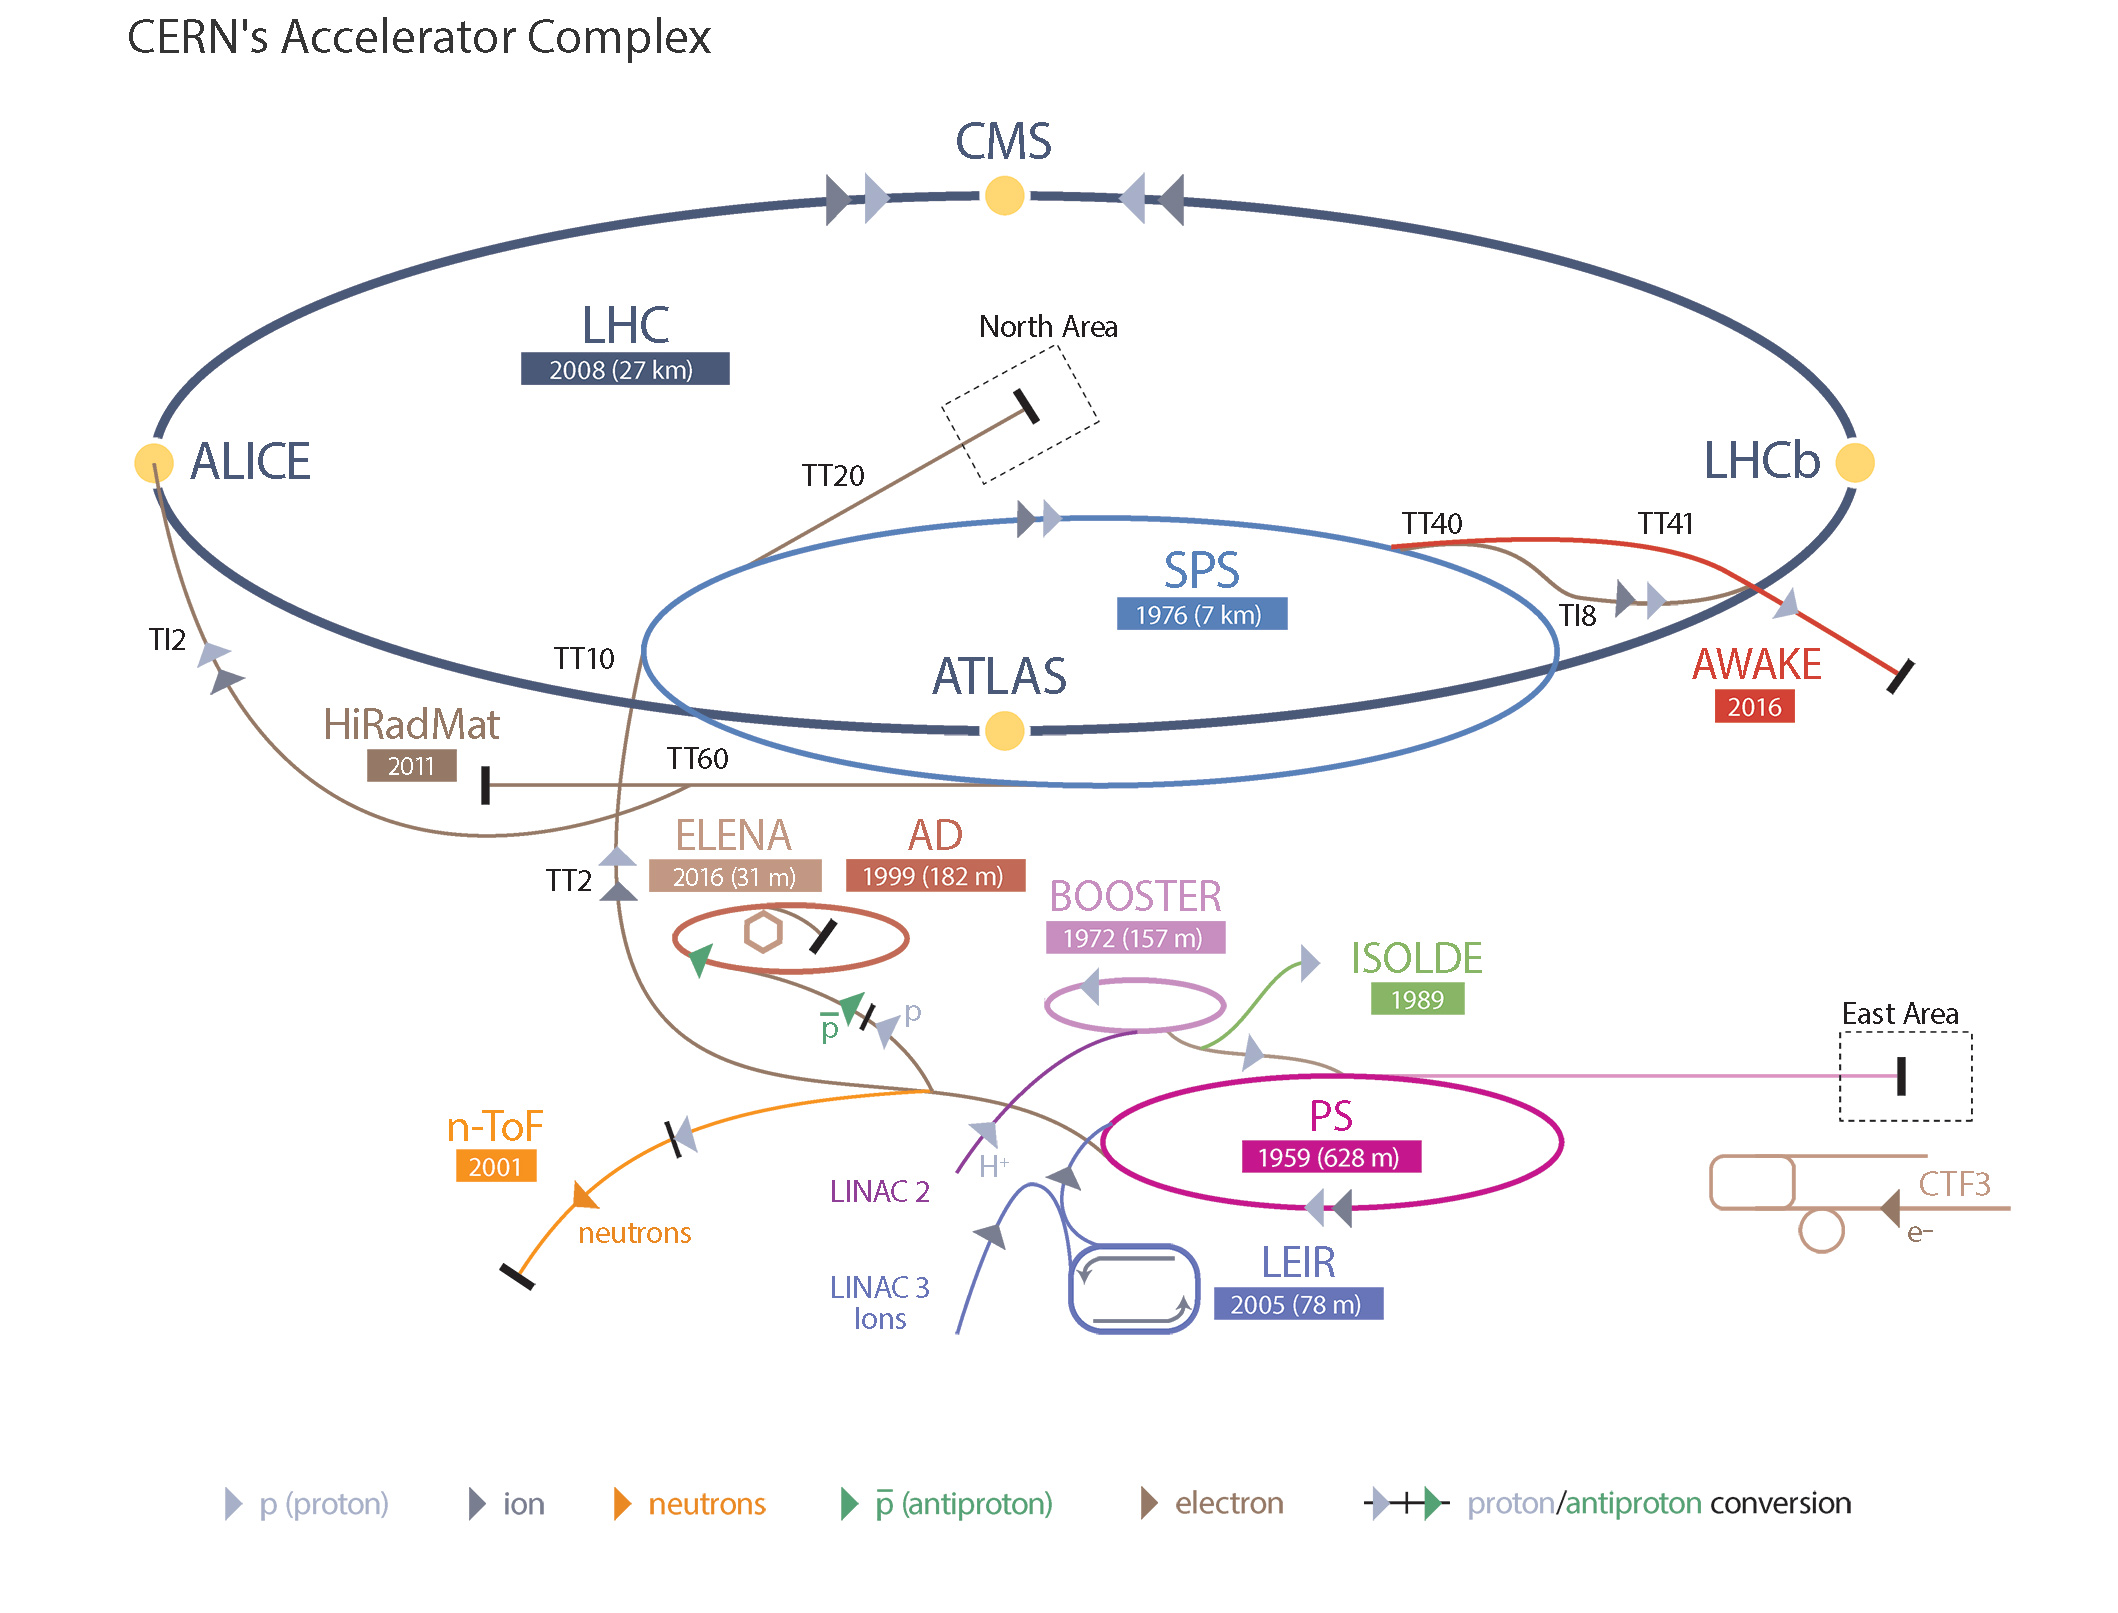
\includegraphics[width=\linewidth]{figures/detector_chapter/LHCRing.png}
  \caption{The infrastructure of the LHC accelerator ring, including the SPS and LINAC2. \ref{LHC}}
  \label{fig:LHC}
\end{figure}

The tight bunching of protons by the LHC ring allows the collider to deliver collisions at a high luminosity, a measure of the number of expected collision events per unit of beam area. Luminosity is measured in both instantaneous and integrated form (i.e., 'luminosity per unit time' and total luminosity delivered to date'); as of the end of the second major LHC run, the collider has delivered a total integrated luminosity of $139 fb^{-1}$, equivalent to approximately $1.39*10^{41}$ collisions per square centimeter \ref{current lumi}. 

At the time of this writing, the LHC is nearing the end of 'Long Shutdown 2' (LS2), a two-year long upgrade period designed to increase detector performance and lay the groundwork for the upcoming high-luminosity LHC (HL-LHC) upgrade, which is slated to begin in approximately 2027 and aims to increase the design luminosity of the LHC by at least a factor of 5 \ref:{HL-LHC}. Higher luminosity allows for the production of more rare physics events, but also dramatically increases the incidence of unwanted "pileup" events; mitigating this is one of the major efforts of the CERN physics community during the lead-up to the HL-LHC run.

The LHC ring accelerates beams to a center-of-mass collision energy of 13 TeV. The ring consists of two primary beam pipes, one containing a "clockwise" beam and the other containing a "counterclockwise" beam, which overlap at the four primary collision points. These correspond to the four major LHC physics experiments: ATLAS  \ref{ATLAS_prop} and CMS \ref{CMS}, which are "general purpose" physics detectors, LHCb \ref{LHCb}, which is specialized to study the physics of hadrons containing bottom (or "beauty") quarks, and ALICE \ref{ALICE}, which is primarily designed for heavy-ion physics. Due to the highly sensitive nature of their instrumentation, these detectors are buried approximately 100 meters underground to avoid interference from high-energy cosmic rays.

\section{The ATLAS Detector} \label{sec:ATLAS} 

The work contained in this dissertation was performed using the ATLAS (A Large Toroidal LHC ApparatuS) detector. Together with its "sibling detector" CMS (the Compact Muon Solenoid), the ATLAS detector is one of CERN's two "general purpose" detectors, so-called because it is designed to observe a wide variety of high-energy physics phenomena. The ATLAS detector is cylindrical, with a diameter of 25 meters and a length of 44 meters \ref{ATLAS}. Upon colliding at the interaction point in the center of the detector, the constituent particles of each proton will interact with one another through a host of different physical processes, producing a variety of new particles traveling at high velocities. The ATLAS detector is comprised of several specialized subsystems, each of which is responsible for logging different properties of these decay products. Each of these subsystems is optimized to detect specific properties of a collision event; taken together, they provide a detailed snapshot of the moment of interaction.
	The Inner Detector (ID), a high-resolution detector composed of primarily of silicon, measures the tracks of particles close to the primary vertex. It is encased within a 2T solenoidal magnetic field that bends the tracks of charged particles produced at the collision point, allowing particle momenta to be measured as a function of the curvature of their trajectories. Enclosing the Inner Detector are two nested calorimeter systems: a liquid-argon-and-lead electronic calorimeter (ECAL) that measures the energy of incident photons and electrons, and a primarily scintillator-tile-and-steel hadronic calorimeter (HCAL) that measures the energy of hadronic showers. Finally, a muon spectrometer composed of gas-filled tubes and chambers records the tracks of muons, which do not decay in the calorimeters like most other particles \ref{muons}.
	The entirety of the muon spectrometer is suffused with magnetic field generated by 24 toroidal magnets, eight of which lie in the barrel, generating a field of 1T and eight of which lie in each endcap, generating a field of 0.5T \ref{Diehl Muons}. These magnets bend the trajectories of muons in a manner similar to the inner solenoidal magnet system, allowing the momenta of particles to be measured based on the track curvature. The ATLAS detector is also equipped with a highly sensitive trigger system, which uses a wide variety of physics signatures in each of these detector subsystems to determine which collision events to store for later analysis \ref{ATLAS TDR}. A diagram of the ATLAS detector is shown in figure \ref{fig:ATLAS}.

\begin{figure}
  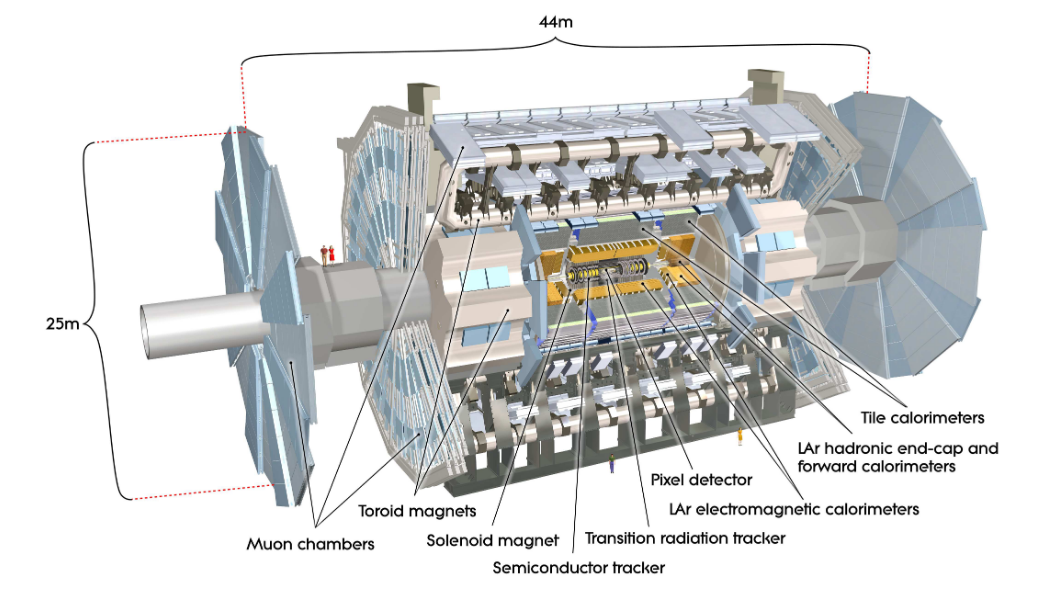
\includegraphics[width=\linewidth]{figures/detector_chapter/ATLAS.png}
  \caption{A diagram of the various subsystems of the ATLAS detector. \ref{ATLAS}}
  \label{fig:ATLAS}
\end{figure}

	The ATLAS detector uses a right-handed coordinate system, with the central interaction point at z = 0. The x-axis points from the interaction point to the center of the LHC ring, while the y-axis points upward. However, particle trajectories are more commonly measured not in (x,y,z) coordinate space but utilizing angular variables ($r$ and $\phi$) in the transverse plane and pseudorapidity $ \eta $ in the longitudinal plane, where $ \eta = -ln(tan( \theta /2) ) $ . This is illustrated in figure \ref{fig:coords}.

\begin{figure}
  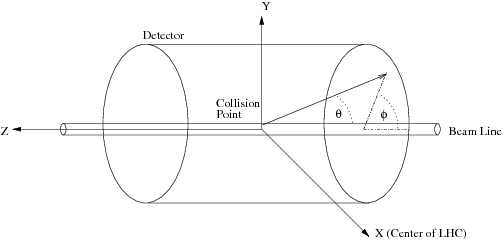
\includegraphics[width=\linewidth]{figures/detector_chapter/coords.png}
  \caption{The coordinate system used to define the ATLAS detector geometry. \ref{cds.cern.ch/record/1699952/plots}}
  \label{fig:coords}
\end{figure}

\subsection{Inner Detector} \label{sec:ID} 

The Inner Detector is composed of five highly granular subdetectors. The closest to the beam, the silicon-based Insertable B-Layer, was added between the LHC's first and second runs in order to improve precision track-vertex measurement for tasks such as b-hadron tagging and tau lepton identification \ref{IBL TDR}, methods discussed more in section \ref{section:tagging}. Proceeding outward from the IBL are the silicon-based Pixel detector and Semiconductor Tracker (SCT), followed by the gas-based Transition Radiation Tracker (TRT) \ref{ATLAS}. The inner detector is encased within a solenoidal magnetic field which causes charged particle tracks to bend according to their charge, as detailed in \ref{sec: Magnets}.

The IBL is composed of 26,880 250×50 $ \mu m^2 $ silicon pixels arranged in an 80 column by 336 row geometry. The pixel modules are supported by 14 support staves, tilted at approximately 14 degrees from the nominal to achieve near-complete cylindrical coverage of the barrel region. The IBL is approximately 33.25 mm from the beam axis, necessitating a replacement of the beryllium beam-pipe with a smaller-radius one for detector reintegration \ref{IBL TDR}.

Silicon is an optimal material for precision trackers due to its status as a semiconductor. Silicon wafers can be easily "doped" with atoms of other elements, leading them to carry either an excess of electrons (n-type semiconductors) or a deficit of electrons (p-type semiconductors). By putting the two together, an n-p junction is formed, leading to a one-way current gate known as a diode. A voltage is then applied to the diode to halt current flow ("reverse biasing"). When ionizing particles such as those produced in collisions pass through the silicon, they will produce a cascade of charge carriers that will induce a current in the diode, which can then be measured by the precision front-end electronics attached to the silicon wafers \ref{Knoll Radiation Detection}.

The pixel detector is similarly composed of silicon pixels, each of which is either 50x400 $ \mu m^2 $ (nominal) or 50x600 $ \mu m^2 $ (near the front-end readout electronics due to spatial constraints). The detector contains 1744 identical pixel sensors, each of which contains 47232 pixels. Three layers of pixels in the barrel region sit at r = 50.5,  88.5 and 122.5 mm from the beam axis, while three layers of pixels in the endcap region sit at r= 495, 580, and 650 mm from the beam axis. The silicon wafers in the pixel detector are "n+ type" strips (n-type semiconductors with extra doping) embedded in an n-type bulk, rather than the traditional n-type and p-type semiconductors due to the fact that excessive radiation from the beam can cause standard n-and-p-type semiconductors to change into one another \ref{Pixel}. 

The SCT is composed of longer silicon microstrip wafers made out of standard n-p type semiconductors. It consists of four layers of 2112 total silicon microstrip modules in the barrel region and 1976 microstrip modules in the endcap regions, with 770 microstrips per sensor module. The strips are 12cm long and 80 $\mu$m wide; the distance of modules from the beam pipe ranges from radii of r= 299 mm to r= 514 mm in the barrel and r=852.8 mm to r= 2720.2 mm in the endcaps. The SCT is designed using less-costly materials than the TRT and IBL, but serves a valuable complementary function \ref{SCT}.

Finally, the TRT consists of polyimide "straws" filled with a gas mixture (70\% Xenon, 27\% Carbon Dioxide, and 3\% Carbon Tetrafluoride), each 4mm in diameter and 144 cm long. In the center of each straw tube is a 31 $\mu$m in diameter grounded gold-plated tungsten wire filament that serves as an anode. Charged particles travelling through the gas medium will ionize it, producing a cascade of ions that will drift to the anode wire. The TRT is uniquely designed to detect low-energy X-ray transition radiation photons, which allows for better identification of electron candidates \ref{TRT}. The barrel region consists of 73 layers of sensor modules ranging from r= 554 mm to r = 1082 mm from the beam pipe, while the encaps straws, arranged in a "wheel" shape, stretch from r= 852.8 mm to r= 2720.2 mm from the beam pipe. 

Additionally, two Minimum Bias Trigger Scintillators, composed of plastic scintillator tiles, sit on the circular endcaps of the ID in order to provide trigger capabilities in the forward region $ |\eta| > 2.5 $. The MBTS endcap scintillator consists of 2 cm thick polystyrene scintillator disks mounted on each endcap at a distance of 3.6m from the collision point at . 

Together, these subsystems form the ATLAS detector's Inner Detector. Each subdetector has a different spatial resolution- the IBL has a resolution of  approximately 10 $\mu m$, the pixel detector has a resolution of 12 $\mu m$, the SCT has a resolution of 16 $\mu m$, and the TRT has a resolution of 130 $\mu m$. The combined effect of these subdetectors is thus to record particle tracks produced in collisions with very high granularity within the range $ | \eta | < 2.5$, allowing for sophisticated physics analyses to be performed. 

\begin{figure}
  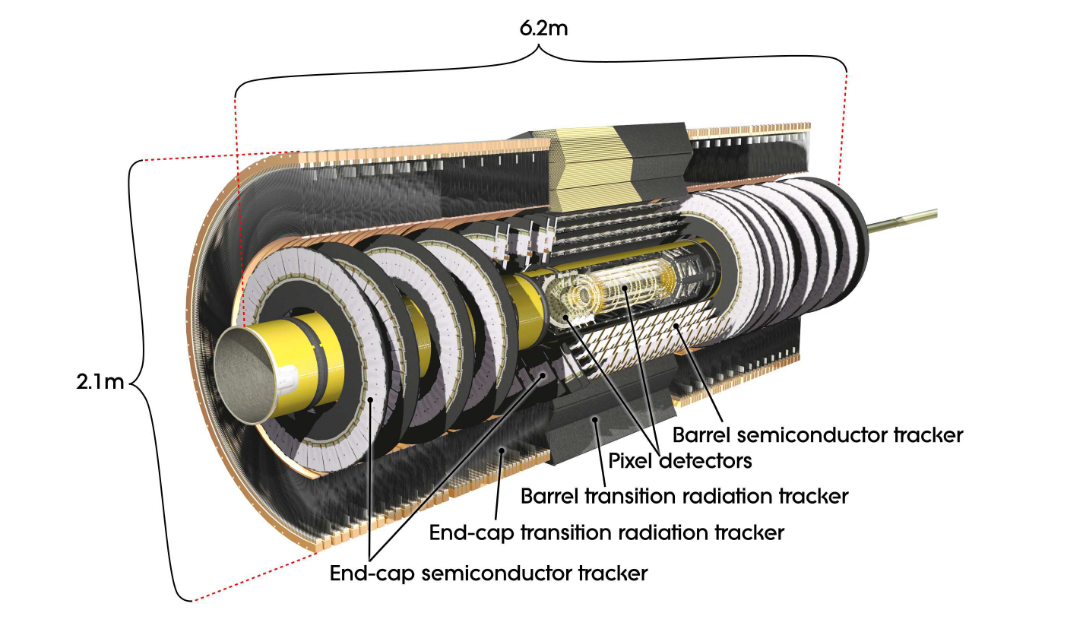
\includegraphics[width=\linewidth]{figures/detector_chapter/ID.png}
  \caption{An illustration of the Inner Detector. \ref{ID}}
  \label{fig:ID}
\end{figure}

\subsection{Solenoid Magnet} \label{sec:solenoid}

Track-bending in the Inner Detector is performed by a solenoid magnet providing a field of 2T throughout the ID bulk. The solenoid magnet is constructed of a single layer of high-strength aluminum-stabilized Nb/Ti conductor. The magnetic field it provides is axial (in the $z$ direction), and thus the direction of bending of charged tracks in the ID is in the $\phi$ direction. 

\subsection{Calorimeters} \label{sec:Calos} 

Measurement of particle energies is performed by the ATLAS detector's two calorimeters. Both calorimeters provide a wider $\eta$ coverage than the Inner Detector, allowing for measurement of hadronic jets and electromagnetic showers that fall outside the $|\eta| < 2.5$ precision tracking range. The liquid-argon based calorimeters function differently than the silicon-based tracking Inner Detector: they do not require the incident particles to be charged, and record energies of particles as they shower (decay) in the calorimeter material rather than simply recording their tracks as they pass through. Broadly speaking, there are two types of calorimeters: homogeneous calorimeters, which are composed entirely of active "measuring" material such as liquid argon or polystyrene scintillator tile, and sampling calorimeters, which interleave layers of this active material with slabs of material designed to cause the incident particles to shower \ref{Misconceptions About Calorimetry}. Both the electronic and hadronic calorimeters are sampling calorimeters; however, they utilize different materials in both the active and non-active layers of the calorimeter. A diagram of the calorimeter system is shown in figure \ref{fig:Calos}.

\begin{figure}
  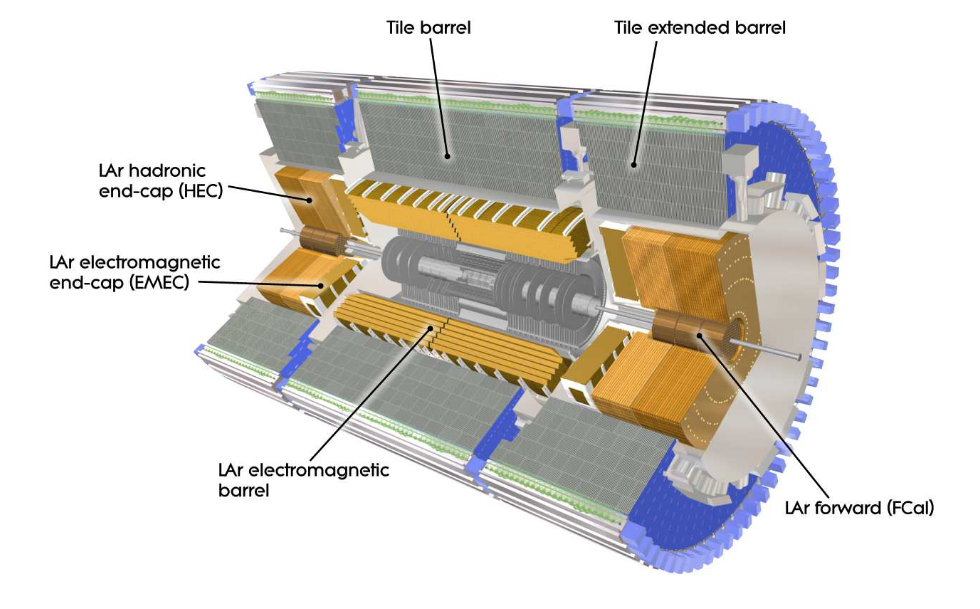
\includegraphics[width=\linewidth]{figures/detector_chapter/Calos.png}
  \caption{An illustration of the ATLAS calorimeter systems. \ref{Calos}}
  \label{fig:Calos}
\end{figure}


\subsubsection{ECAL} \label{sec:ECAL} 

When electrons and photons enter the non-active layer of a sampling calorimeter, they interact with the electric fields produced by the atoms of the layer material and produce showers of bremsstrahlung photons and electron-positron pairs, which then produce electrical signals in the Liquid Argon active layers that are read out by specialized electrodes. The depth of the electronic calorimeter thus must be chosen carefully in order to capture the entirety of a typical EM shower (measured in "radiation lengths" $X_0$, this varies depending on the absorber material). All ECAL subsystems are made of the same materials: liquid Argon (LAr) sampling layer with lead-plate absorber layers, arranged in a unique "accordion" geometry that gives the ECAL complete coverage in $\phi$ . Due to the high atomic number of lead, the electron clouds of the atoms of the absorber plates are well-populated, thus leading to a high likelihood that photons or electrons will shower within the calorimeter bulk.

The ATLAS electronic calorimeter consists of two primary subsystems: one barrel calorimeter, covering $ |\eta |<1.475$, and two end-cap calorimeters, covering $ 1.375<| \eta |< 3.2 $. The barrel calorimeter is composed of two identical half-barrels, separated by a 4mm horizontal gap at z=0, along the plane of the beam pipe. The lead absorber plates, readout electrodes, and "honeycomb" spacers that form the cavities for the liquid argon layer are all zigzag-shaped and arranged in a circular "starburst" pattern around the barrel \ref{ATLAS Liquid Argon TDR}, as depicted in figures \ref{fig:KriegerECALphoto} and \ref{fig:ECALdiagram}. Each half-barrel consists of 1024 accordion absorbers with their associated interleaved spacers and electrodes, weighs 57 tons, and is 3.2 m long, with an inner radius of 2.8 m and an outer radius of 4.0 m. There are three layers of absorbers in the inner precision-measurement region $(0 <| \eta |< 1.35)$ of the barrel and two in the higher-$\eta$ region $(1.35 < | \eta |<1.475)$, each with a different segmentation; the angle, lateral orientation and length of the accordion waves varies with $\eta$.

\begin{figure}
  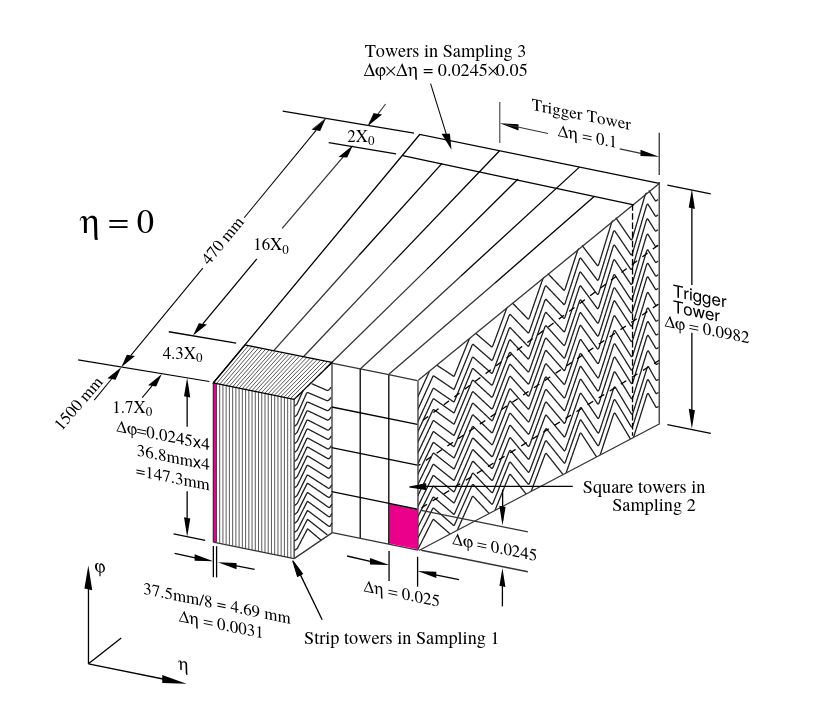
\includegraphics[width=\linewidth]{figures/detector_chapter/ECALdiagram.png}
  \caption{A cutaway diagram of the barrel ECAL deptcting the "accordion" absorber geometry \ref{ECALdiagram}}
  \label{fig:ECALdiagram}
\end{figure}

\begin{figure}
  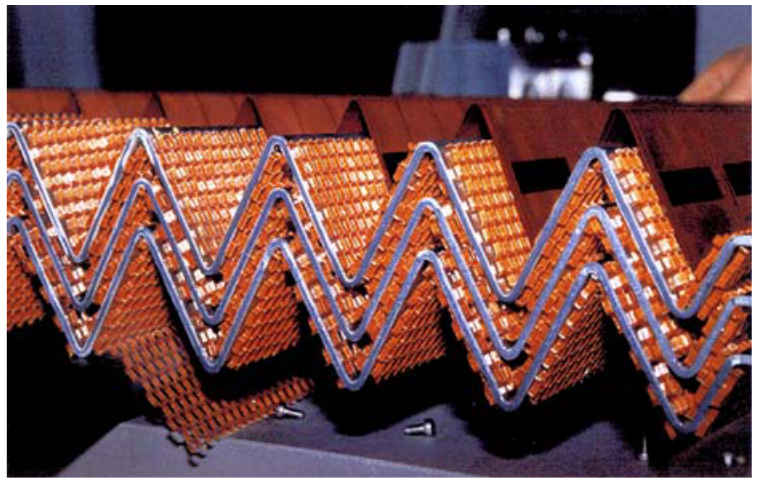
\includegraphics[width=\linewidth]{figures/detector_chapter/ECALphoto.png}
  \caption{A photograph of an ECAL absorber. \ref{KriegerECALphoto}}
  \label{fig:ECALphoto}
\end{figure}

Each end-cap calorimeter is composed of two wheels, one large outer wheel covering $ 1.375<| \eta |<2.5 $, and one smaller inner wheel covering the range $ 2.5<| \eta |<3.2 $. Each endcap is 63 cm thick, weighs 27 tons, and contains 768 accordion absorbers in the outer wheel and 256 absorbers in the inner wheel. Like the barrel, the calorimeter structure in the endcaps consists of three layers of absorber modules in the region nearest the beam pipe in the outer wheel $( 1.5 < |\eta | <2.5 )$ and only two layers both nearest the edges of the outer wheel $(1.375 < |\eta | < 1.5)$ and in the entirety of the inner wheel. In the endcaps, the "zigzag" accordion folds are oriented longways, in the z-direction \ref{Discussion on the electromagnetic calorimeters of ATLAS and CMS}.

In the barrel, each absorber is at minimum 22 radiation lengths thick (though this varies up to 33 radiation lengths as a function of pseudorapidity $\eta$), thus ensuring that electromagnetic showers are contained within the calorimeter bulk. In the endcaps (except for the outer wheel edge region  $ 1.375< | \eta |< 1.475 $), the calorimeter systems are at minimum 24 radiation lengths thick.

In addition to the accordion sampling layer folds of the ECAL bulk, a presampler detector composed of 64 modules in the barrel and 32 in each endcap provides information about electromagnetic objects before they enter the sampling calorimeter. The presampler modules consist of interleaved electrodes between glass-fiber composite plates, filled with liquid argon in the gaps. In the barrel, the presampler is 11mm thick and covers the entire barrel range; in the endcaps, the presampler is 4mm thick and covers the range $(1.5<| \eta |<1.8)$ \ref{Presampler}.

\subsubsection{HCAL} \label{sec:HCAL} 

Hadronic showers typically have both electromagnetic and non-electromagnetic components, and, as such, are typically much larger than electromagnetic showers  As such, the hadronic calorimeter is required to be much deeper than the electronic calorimeter, in order to longitudinally contain hadronic showers in their entirety. The characteristic length scale for hadronic showers is the nuclear interaction length ($\lambda\_{int}$), which can be up to 30 times larger than the radiation length $X_0$. The ratio $\lambda\_{int} / X_0 $ is proportional to atomic number; thus, placing at least one layer at the front of a hadronic calorimeter that uses a high-atomic number material such as lead in its absorbers is essential in order to distinguish between purely electromagnetic showers and the electromagnetic components of hadronic showers. For the ATLAS detector, this purpose is served by the ECAL: a significant fraction of the energy of hadronic jets is deposited in the ECAL as electromagnetic activity due to the presence in jets of charged hadrons such as pions. In deeper layers, calorimeter absorbers should be constructed of a dense material such as iron or steel, so that hadrons are able to interact with the nuclei of absorber-layer atoms and produce signals in the active layers \ref{Misconceptions About Calorimetry}.  

The ATLAS HCAL is composed of three major subsystems: the TileCal, which uses polystyrene scintillator tiles in the active layer and steel in the absorber layer; the LAr endcap calorimeters, which use liquid argon as the active layer and copper as the absorbers; and the LAr forward calorimeters, which use liquid argon as the active layer and contains both copper and tungsten absorber layers.

The TileCal is located immediately behind the electronic calorimeter, and covers the pseudorapidity range $|\eta |< 1.7$. It consists of a central barrel region and two extended barrel regions, one on each side of the detector cylinder, as depicted in figure \ref{fig:TileCalDiagram}. The central barrel is 5.8 m long and each extended barrel is 2.6m long; all three have an inner radius of 2.28m and an outer radius of 4.25m. This corresponds to a total radial depth of approximately 7.4 $\lambda\_{int}$. Additionally, each subsystem is composed of 64 wedge modules, each spanning $5.625 ^{\circ}$ in $\phi$ . Each wedge consists of a series of trapezoidal scintillator tiles (3mm thick, but varying in width and height depending on position in the wedge) interleaved with steel absorber; two fiber-optic cables connect each scintillator tile to two photomultiplier tubes in order to enable accurate readout. Each tube connects to multiple tiles; these readout channels are structured in order to form a system of calorimeter cells. 

\begin{figure}
  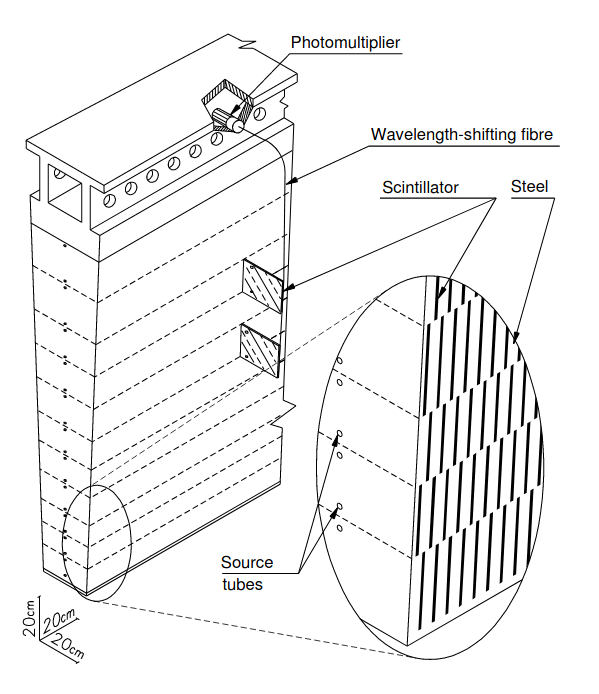
\includegraphics[width=\linewidth]{figures/detector_chapter/TileCal.png}
  \caption{A diagram of the TileCal geometry \ref{TileCal}}
  \label{fig:TileCalDiagram}
\end{figure}

When ionizing particles produced by interactions in the steel absorber reach the scintillator tiles, they produce ultraviolet light. The scintillator tiles are composed of polystyrene doped with 1.5\%  p-terphenyl (PTP) and 0.044\% 1,4-bis(5-phenyloxazol-2-yl) benzene (POPOP), which serve to shift the ultraviolet photons into visible light. These are then read out through the photomultiplier tubes \ref{ATLAS}.

The Hadronic Endcap Calorimeter (HEC) uses flat copper plates as the absorber layer and liquid argon as the active material, and covers the range  $1.5 < | \eta | < 3.2 $. It consists of two wheels in each endcap, each wheel containing two longitudinal sections. Each wheel is cylindrical with an outer radius of 2030 mm, and consists of 32 identical wedge modules. The front wheels contain 24 copper plates each; the rear wheels contain 16 each.

Finally, the LAr forward calorimeters (FCAL) sit in the very forward region closest to the beamline, $3.1<|\eta |< 4.9$, and are designed to measure the energy of very forward, often low-energy hadronic jets.  The FCAL is unique in that, due to its forward position, it experiences a very large particle flux; it uses very thin active layers in order to mitigate the potential ion buildup this may cause.  The FCAL contains three subdetectors, labelled FCAL1, FCAL2 and FCAL3 proceeding outward from the beamline.

Because it lies outside the eta range of the electromagnetic calorimeter, the FCAL must also contain an electronic calorimeter component in order to capture the electronic components of hadronic showers. FCAL1 is this electronic calorimeter, and uses copper as its active material. It is composed of a matrix of copper plates with circular holes in them, through which are pushed copper electrode rods utilized for readout. The gap between these rods and the plates is then filled with LAr; this setup offers very fine control over the active layer thickness. This can be seen in figure \ref{fig:FCAL}.

\begin{figure}
  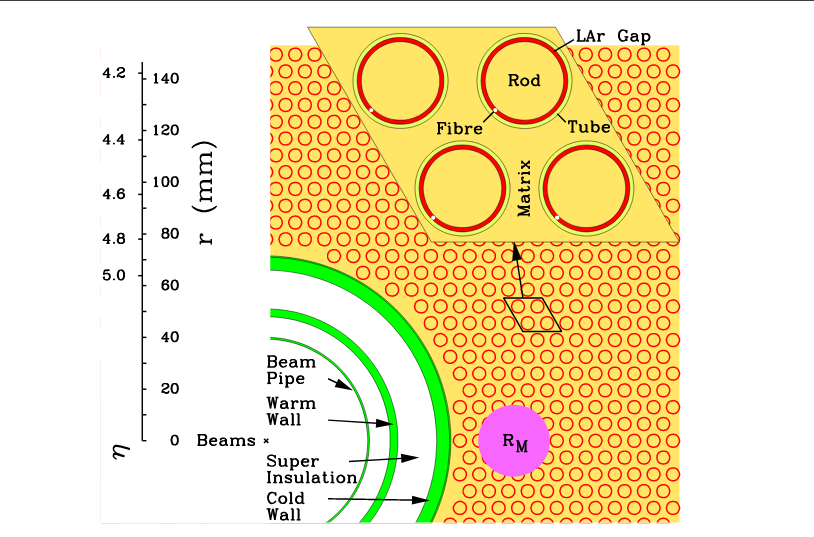
\includegraphics[width=\linewidth]{figures/detector_chapter/FCAL.png}
  \caption{A diagram of the FCAL geometry \ref{ECALTDR}}
  \label{fig:FCALDiagram}
\end{figure}


FCAL2 and 3, however, are optimized for the much longer characteristic shower scales of hadronic interactions. They are set up identically to FCAL1, but use tungsten readout electrode rods instead of copper \ref{ECALTDR}.

\subsection{Toroid Magnets} \label{sec:toroids}

A series of three large toroid magnets (one in the barrel and one in each endcap) are designed to curve the tracks of muons in the muon spectrometer, allowing for their momentum to be measured using their curvature. Each toroid consists of eight rectangular air-core coils, wound in the $R - z$ plane. Barrel and endcap toroids are rotated at an angle of $22.5 ^{\circ}$ with respect to each other in order to provide maximal coverage. Because the toroidal magnets are toroids and lie in the $R - z$ plane, they curve tracks in this plane as well; this is distinct from the solenoid, which curves tracks in $\phi$.

Each barrel toroid magnet consists of a "racetrack-style" Aluminum-stabilized Nb/Ti/Cu conductor wound into two double pancakes; together, these supply a field bending-power ranging from 1.5 to 5.5 Tm  in the pseudorapidity range  $0 < |\eta | < 1.4$ \ref{Cold Mass Integration of the ATLAS Barrel Toroid}. Endcap toroids are similarly constructed racetrack-style magnets, but are bolted and glued together with eight keystone wedges in order to withstand the Lorentz forces and hold the magnets together. Endcap toroids supply a bending-power of 1 Tm to 7.5 Tm in the range $ 1.6 < |\eta | < 2.7 $ \ref{Engineering status of the superconducting end cap toroid magnets for the ATLAS experiment at LHC}.

\subsection{Muon Spectrometer} \label{sec:Musyst}
 
Unlike electrons and photons, muons are not stopped by the electronic calorimeter. This is due to the fact that a charged particle's energy loss as a function of unit distance due to bremsstrahlung is proportional to its energy and inversely proportional to the square of its mass; because muons are much heavier than electrons, this energy loss drops off substantially at the energies seen at the LHC. While at very high energies, muons again begin to lose most of their energy due to radiation, this occurs at muon energies exceeding a few hundred GeV. Thus, while muons may lose some energy in the electronic calorimeter, and at high energies may be slowed substantially, it is typically not enough to cause them to come to a stop \ref{Muon Stopping}. 

Similarly, because muons do not interact through the strong nuclear interaction, like pions and other hadrons, they are not stopped by the high-Z material of the hadronic calorimeter. Thus, muons in ATLAS are "minimum ionizing particles", that is, particles that lose energy when travelling through material primarily through the process of ionization \ref{PDG}. Therefore, a specialized detector subsystem must be built to measure the energies of muons exiting the detector.

The Muon Spectrometer, is, as its name suggests, not a calorimeter, but a device designed to measure the momentum spectra of outgoing muons (from which their energies can be calculated). It consists of four major types of detector chambers, two designed for muon tracking and two designed for triggering. A cutaway diagram of the full Muon Spectrometer is shown in figure \ref{fig:MuSyst}.

\begin{figure}
  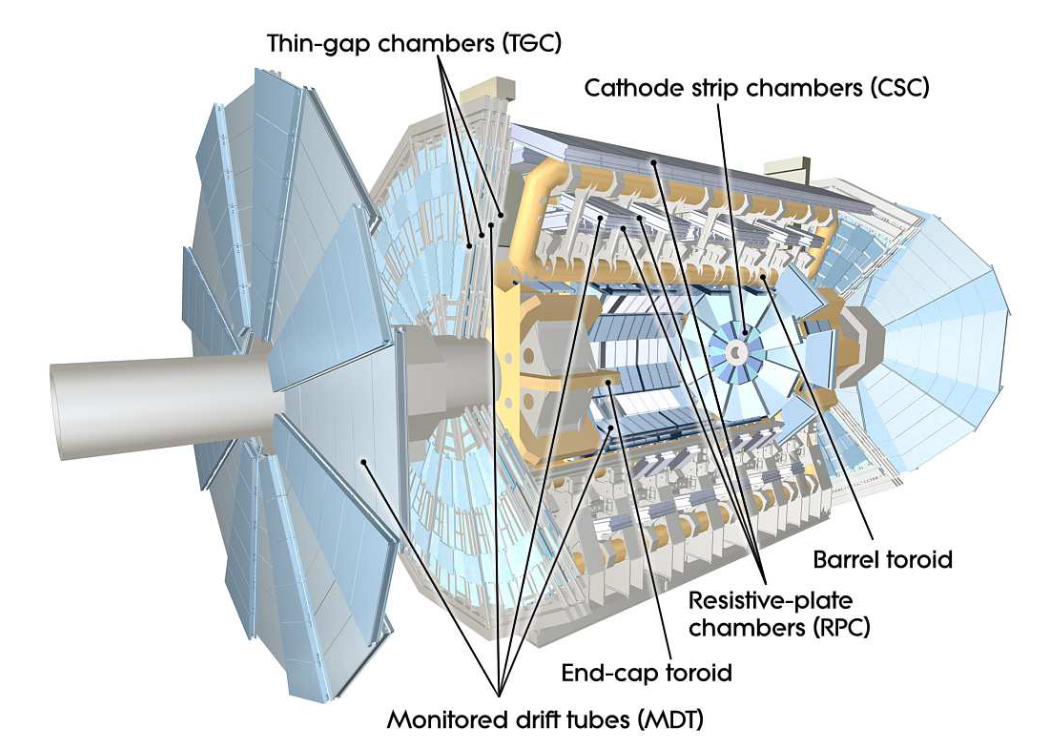
\includegraphics[width=\linewidth]{figures/detector_chapter/MuSyst.png}
  \caption{A diagram of the Muon System \ref{Musyst}}
  \label{fig:MuSyst}
\end{figure}

The primary tracking detectors are the Monitored Drift Tube (MDT) chambers. A single MDT is an aluminum tube 29.970 mm in diameter, threaded through with a 50 $\mu m$ radius tungsten-rhenium wire that is affixed with a stopper at each ends. The tube is pumped through with a mixture of 93\% argon gas and 7\% carbon dioxide, held at a pressure of three bars. Each anode wire is held at a potential of 3080 V, while each tube exterior serves as a cathode, and is grounded. As a muon passes through the tube, it will ionize the gas within; the electrons thus produced will drift to the high-voltage wire and produce electrical signals that can be read out by the specialized boards to which the tubes are attached. Because a muon passing through the tube will leave a trail of ions in its wake, each tube is able to record the minimum radius at which the track passes through the wire, as depicted in figure \ref{fig:MDT}. However, because this in itself is not enough to reconstruct a track, multiple layers of tubes must be placed together to form a chamber module.

\begin{figure}
  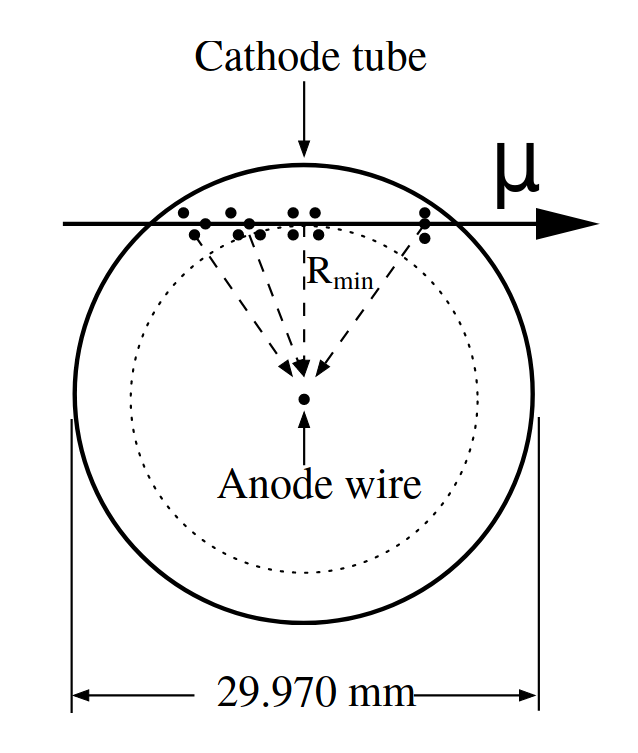
\includegraphics[width=0.5\linewidth]{figures/detector_chapter/MDT.png}
  \caption{A diagram of a Monitored Drift Tube \ref{MDT}}
  \label{fig:MDT}
\end{figure}

There are 18 varieties of MDT chamber modules, each containing a different number of MDT tubes. Each chamber module consists of one or more "multilayers" of tubes, which consist of either three or four layers of tubes vertically separated by 6.5, 170, or 317 mm, depending on their position in the muon spectrometer. In the barrel, chambers are arranged in three concentric rings around the beam axis, at radii approximately 5m, 7.5m, and 10m from the beamline. In the end-cap region, chambers are arranged in large wheels perpendicular to the beam at approximately 7.4m, 10.8m, 14m, and 21.5m from the interaction point. Each MDT chamber has a spatial resolution of approximately 35 $\mu m$. Overall, MDT chambers cover the region $ |\eta | < 2.7$, though the number of chambers intersected varies as a function of $\eta$ \ref{MDTs}. The MDT system geometry is shown in figure ref{fig:MDTChamber}. 

\begin{figure}[ht!]
  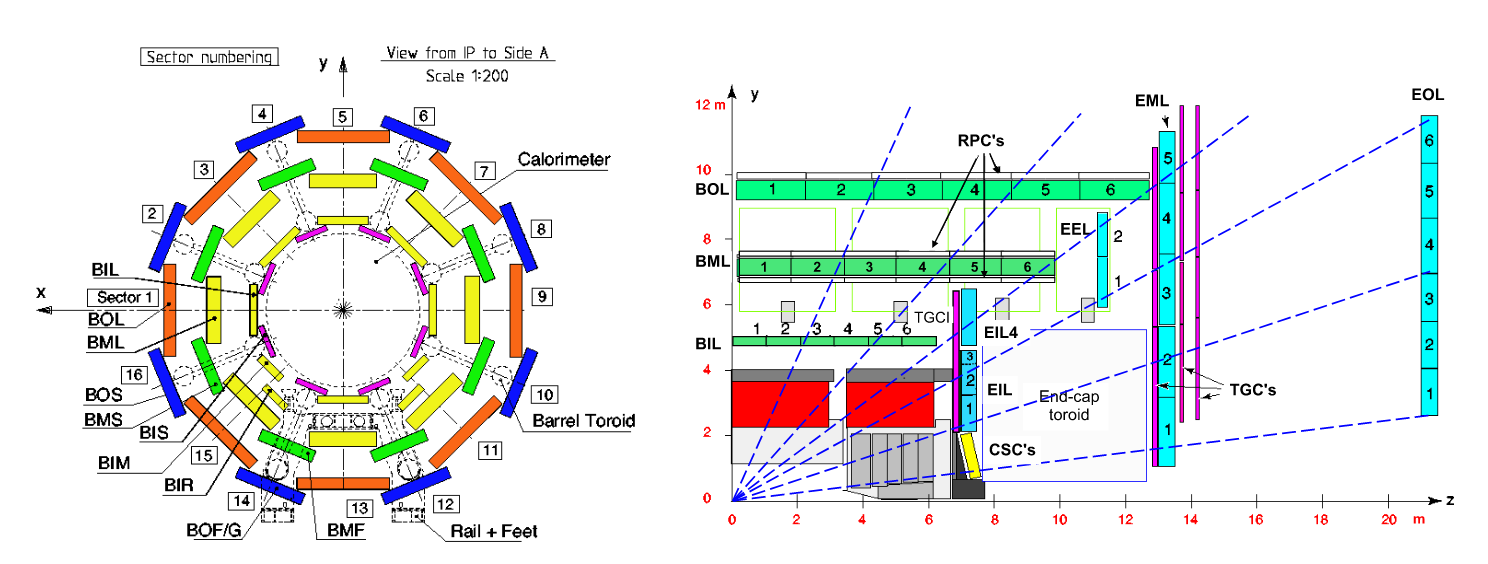
\includegraphics[width=\linewidth]{figures/detector_chapter/MDTChamber.png}
  \caption{A diagram of the MDT chamber geometry from two positions, one looking down the beam pipe and one alongside the detector. \ref{MDT}}
  \label{fig:MDTChamber}
\end{figure}

Closer to the beam, the event rate is higher due to beam halo effects caused by protons decaying into pions (and in turn, muons) in the beam pipe\ref{Boudreau top}. Because the expected rate exceeds the tolerance of the MDT chambers, a different type of muon chamber is situated closer to the beam pipe in order to safely deal with the larger event rate. Cathode Strip Chambers (CSCs), are used in the inner endcap chambers in the range $ 2 < | \eta | < 2.7 $.

Each CSC endcap consist of two circular disks, one containing eight large chambers and one containing eight small chambers. A CSC is a type of multiwire proportional chamber that functions similarly to an MDT: muons passing through the CSC will ionize the $Ar-CO_2$ gas within; electrons will then drift to anode wires and produce a current. Unlike MDTs, however, CSCs are flat, and threaded through with multiple anode wires. Unlike an MDT, a CSC utilizes cathode strips for readout, rather than reading from the anode wire directly: electrons produced during ionization will float to the anode wire; this will produce a charge screening effect that induces a current in the cathode strips. These are then read out; the strength of the current on each strip can be used to determine the path of the muon track.

Each chamber contains eight layers of cathode strips criscrossed with anode wires and filled with a mixture of 80\% argon gas and 20\% $CO_2$. Four of these layers are segmented in the $\eta$ direction and four segmented in the $\phi$ direction, enabling spatial determination of both coordinates of a muon track. Each CSC chamber has a spatial resolution of approximately 40 $\mu m$ in the "bending" $\eta$ plane and 5 mm in the "non-bending" $\phi$ plane. The CSC endcaps are angled slightly toward the interaction point in order to improve resolution; the readout pitch is 5.31mm for the large chambers and 5.66mm for the small ones \ref{CSC}.

In addition to the precision MDT and CSC chambers, the muon system contains a series of chambers designed explicitly for quickly triggering on muon events. These are the Resistive Plate Chambers (RPCs) and Thin Gap Chambers (TGCs). These provide cursory information about the tracks of muons passing through the detector in order to rapidly determine whether an event should be stored for later analysis.

In the barrel region ($| \eta | < 1.05 $), the trigger chambers are Resistive Plate Chambers (RPCs). RPCs are gas-filled detectors, like MDTs and CSCs, but do not contain a wire. Instead, in each RPC gas-gap module, two resistive plates made of plastic laminate are held 2mm from one another and suffused with a large electric field of 4.9 kV/mm. Incoming muons will then produce ionization avalanches that will induce a current on copper anode strips on the outside of the module through capacitive coupling. RPCs are filled with a gas mixture of 94.7\% 1,1,2,2-Tetrafluoroethane (C2H2F4), 5 \% Isobutane (Iso-C4H10) and 0.3\% Sulfur Hexafluoride (SF6). Each RPC chamber consists of four gas-gap modules, segmented in $\phi$ in a manner similar to the CSCs. RPCs follow the same naming scheme as the MDT chambers, and are arranged in three concentric layers around the detector, one small at radii of 7.820 m, 8.365 m, and 10.229m, and one large at radii of 6.800m, 7.478m, and 9.832m.

In the endcaps $(1.05 <|\eta| < 2.4)$ , the trigger chambers are Thin Gap Chambers (TGCs). TGCs serve two purposes: first, to provide trigger capabilities, and second, to complement the radial measurement of the endcap MDT chambers by providing a precision measurement of the $\phi$ coordinate of incoming muon tracks. TGCs are structured very similarly to CSCs, as they are also multiwire proportional chambers. However, TGCs are designed so the wire-to-cathode distance (1.4mm) is smaller than the wire-to-wire distance (1.8mm). TGCs are filled with 50\% $CO_2$ and 45\% n-pentane (n-C5H12); the choice of this gas in addition to the chamber geometry substantially increases the ratio of charges reaching the wire to ionizations produced by the incident particle. Two layers of copper strips in each chamber are segmented in $\phi$ and used as readout channels.

One set of doublet TGC chambers is placed just inside the inner MDT endcap, covering the range $ 1.05 < |\eta| <1.92 $ (divided radially into two concentric non-overlapping "Endcap" and "Small Wheel" regions); three others (one triplet and two doublets) are placed with the middle MDT endcap to form the "Big Wheel" (covering the range $ 1.92 < |\eta| < 2.4$). On the Big Wheel, TGC chambers are arranged in two circular wheels, each split into 12 segments. The outer wheel (further from the interaction point) contains 48 modules, each subtending 7.5 $^{\circ}$, while the inner wheel (coser to the interaction point) contains 24 modules each subtending 15 $^{\circ}$. Each module contains between 3 and 12 TGCs, depending on its position in the wheel. Similarly, the inner TGC layer is also arranged in a wheel shape, and contains a total of 180 TGCs ref{TGCs}. The TGC wheels are depicted in figure \ref{fig:TGCWheel}.

\begin{figure}[ht!]
  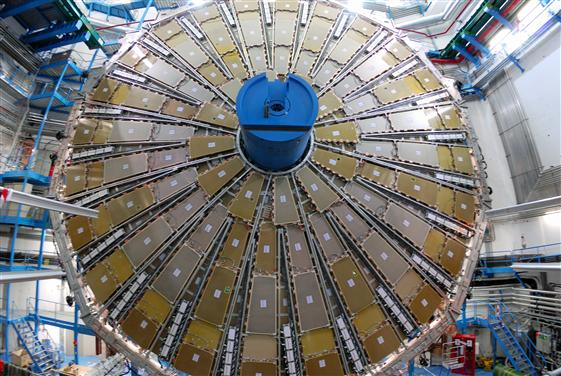
\includegraphics[width=\linewidth]{figures/detector_chapter/TGCWheel.png}
  \caption{A photograph of the TGC wheels. \ref{CERN-EX-0609016}}
  \label{fig:TGCWheel}
\end{figure}

\subsection{Trigger} \label{sec:Trigger}
Due to the high rate of collision events delivered by the accelerator, it is impossible to save the data from every single collision produced in the detector. Luckily, only a subset of these are relevant for physics analysis; indeed, the majority of events produced in the detector are "minimum bias" events caused by low-energy interactions between beam protons that are useful only for performance studies \ref{MBTS}. A three-leveled system of triggers is therefore implemented in order to reduce the event rate from 40 MHz to a more manageable 200 Hz. The trigger system is a mix of both hardware and software based subsystems, and is optimized to balance the demands of complexity and speed: more sophisticated algorithms take more time to run, but this cannot get in the way of more data-taking. Each successive trigger is thus more complex than the last, with the lower-level trigger systems applying coarser selections and the higher-level triggers applying finer ones \ref{trigger}.

The first tier of trigger systems, called the L1 trigger, is hardware-based. It utilizes information directly received from the detector subsystems to search for a variety of noteworthy physics objects: high-transverse-momentum muons (transverse momentum here meaning the component of the momentum in the radial coordinate, denoted by $p_T$) are identified using the RPC and TGC chambers discussed in section \ref{sec:Musyst}, while photons, electrons, tau leptons, and hadronic jets are identified using coarse calorimeter information. These triggers form the "L1Muon" and "L1Calo" trigger menus; this information in addition to that of other subsystems such as the MBTS are then sent to the Central Trigger Processor (CTP). The CTP then combines the information from these trigger systems and sends it to the L2 trigger; it also indicates spatial regions of interest using a third trigger called "L1Topo" and calculates quantities of interest such as missing transverse energy (here denoted $E_T^miss$, defined as the negative vector sum of the $p_T$ of all objects in the event. $E_T^miss$ serves as an indicator of the presence of unobserved neutrinos or other "invisible" decay products in the event). The combined activity of the L1 triggers serve to reduce the event rate to less than 1kHz.

After passing the hardware-based L1 trigger, events then proceed to the software based L2 trigger and Event Filter, which are known together as the High Level Trigger (HLT). HLT triggers utilize a full-granularity event display in order to perform trigger calculations, analyzing the regions of interest marked by the L1 triger. It is at the HLT stage that reconstruction and matching of tracks using Inner Detector information, as well as jet, photon and electron object identification and tagging of objects such as b-jets and tau leptons is performed. All events that pass one or more triggers in the HLT menu are recorded, reducing the event rate to the aforementioed 200 Hz. Triggers may also be 'prescaled' (for which only a set fraction of the events that pass are recorded);this allows analyzers to explore properties of events that normally occur at a rate much higher than can be handled by the trigger system. The triggers utilized in the analyses described in this dissertation are detailed in section \ref{sec:} and \ref{sec:}.

